\documentclass{article}
\usepackage[UTF8]{ctex}
\usepackage{geometry}
\usepackage{float}
\usepackage{fancyhdr}
\usepackage{extramarks}
\usepackage{amsmath}
\usepackage{amsthm}
\usepackage{amsfonts}
\usepackage{tikz}
\usepackage{multicol}
\usepackage[ruled,vlined]{algorithm2e}
\usepackage{algpseudocode}
\usetikzlibrary{automata,positioning}

\geometry{top = 2cm, bottom = 2cm}

\author{黄道吉}
\title{智能笔记本}
\date{\today}

\begin{document}

\maketitle

\section{目的与创新点}


平板电脑以它丰富的功能和便捷的使用体验成为了大学生学习的生产力工具之一。作为电子设备的它用于学习时,天生的可以方便的和学校的教学平台连通取得教师的课件,或是同学之间分享笔记;另一方面,它笔记本式的外形配合手写笔既能贴合传统书写的体验,又便于随身携带。而与这种信息化的学习方式相对照,当今中国的高中生学习仍然处于大量使用纸张和手写的方式中。如果将这种工具整合进高中生的日常学习当中,将会大大便利学习资料的分享,提升学习效率,也能够借用信息化的力量将学生从繁杂的手写任务中解放出来。

因此,我设想了一种整合普通的笔记本和平板电脑的产品来便利高中生的学习。它能够做到
\begin{itemize}
    \item 便利学习资料的信息化:资料录入时有自动的读取,资料云端存档,便捷的师生/生生资料互传
    \item 减轻学生的负担:节省纸张等耗材的消费,降低最终产品的成本
    \item 自然的使用体验:尽量贴合传统纸笔使用习惯,操作简捷
\end{itemize}

我的设想是在现今已经推出的产品的基础上改进和整合的。相较其他的产品,我的设想针对学校的应用场景做了特定的设计,考虑进学生和学校的需求。文章的第二部分将会介绍这些参考的产品的优缺点和值得吸收和改进的地方。第三部分将会介绍具体实现的方案,最后我会讨论一些可能遇到的困难和解决办法。

\section{竞品的优缺点}

一本笔记本是曾经推出过的产品,它整合了笔记本、草稿版和充电宝,整体结构和我设想的产品类似。在左侧有一个布吉板(boogie board),支持按压式的书写和清屏,并不支持部分擦除。右侧可以安防普通的左右翻页的笔记本,这样打开笔记本时会将左侧的布吉板挡住。笔记本外壳有电子锁,支持手势解锁,但在断电时会锁死,只能充电后打开。此外在中间骑缝位置安放了一块电池为电子锁和布吉板供电,也可以用作充电宝,有评测\footnote{https://www.youtube.com/watch?v=Pn4CLxbHR94}显示它的续航并不久。

由于左右侧的板子并不能协作,因此左侧的布吉板并没有最大化发挥它的作用,另外它也不符合我的设想中对信息化的要求。和这款产品相比,我的设想最大化利用了左面草稿版的性能,并借用网络实现学习资料的数据化,减轻对纸质产品的依赖。

柔宇的柔记RoWite笔记本通过在特定的笔记本上书写,可以将书写内容同步到特定的手机应用上,记录书写轨迹,软件端实现了手写字符的识别和云端同步。它需要压感的手写笔,对纸张没有特定要求。但在美版亚马逊的评论\footnote{https://www.amazon.com/RoWrite-Smart-Writing-Pad-RY0201-CF5NA/dp/B07D1C34G6}上有反应它只能用专用的纸,并且扫描效果分辨率并不高,此外也只能在专用app上处理扫描结果,没有很大的自由度。

Wacom 的 bamboo slate也是一款类似的产品,它可以对接Onenote和Evernote来同步,亚马逊上的用户评论反应在翻页时需要按键是很不符合使用习惯的设计。此外moleskine的类似产品通过在笔尖内置摄像头来扫描书写的轨迹,但据称扫描效果并不如压感的产品。

Google的Chromebook是美国的教育市场广泛使用的一款廉价电脑。它的系统支持快速开机、云端同步、管理员的中心管理。我借鉴了它为教育市场而改造出的系统特性。

\begin{figure}[!htb]
\minipage{0.50\textwidth}
  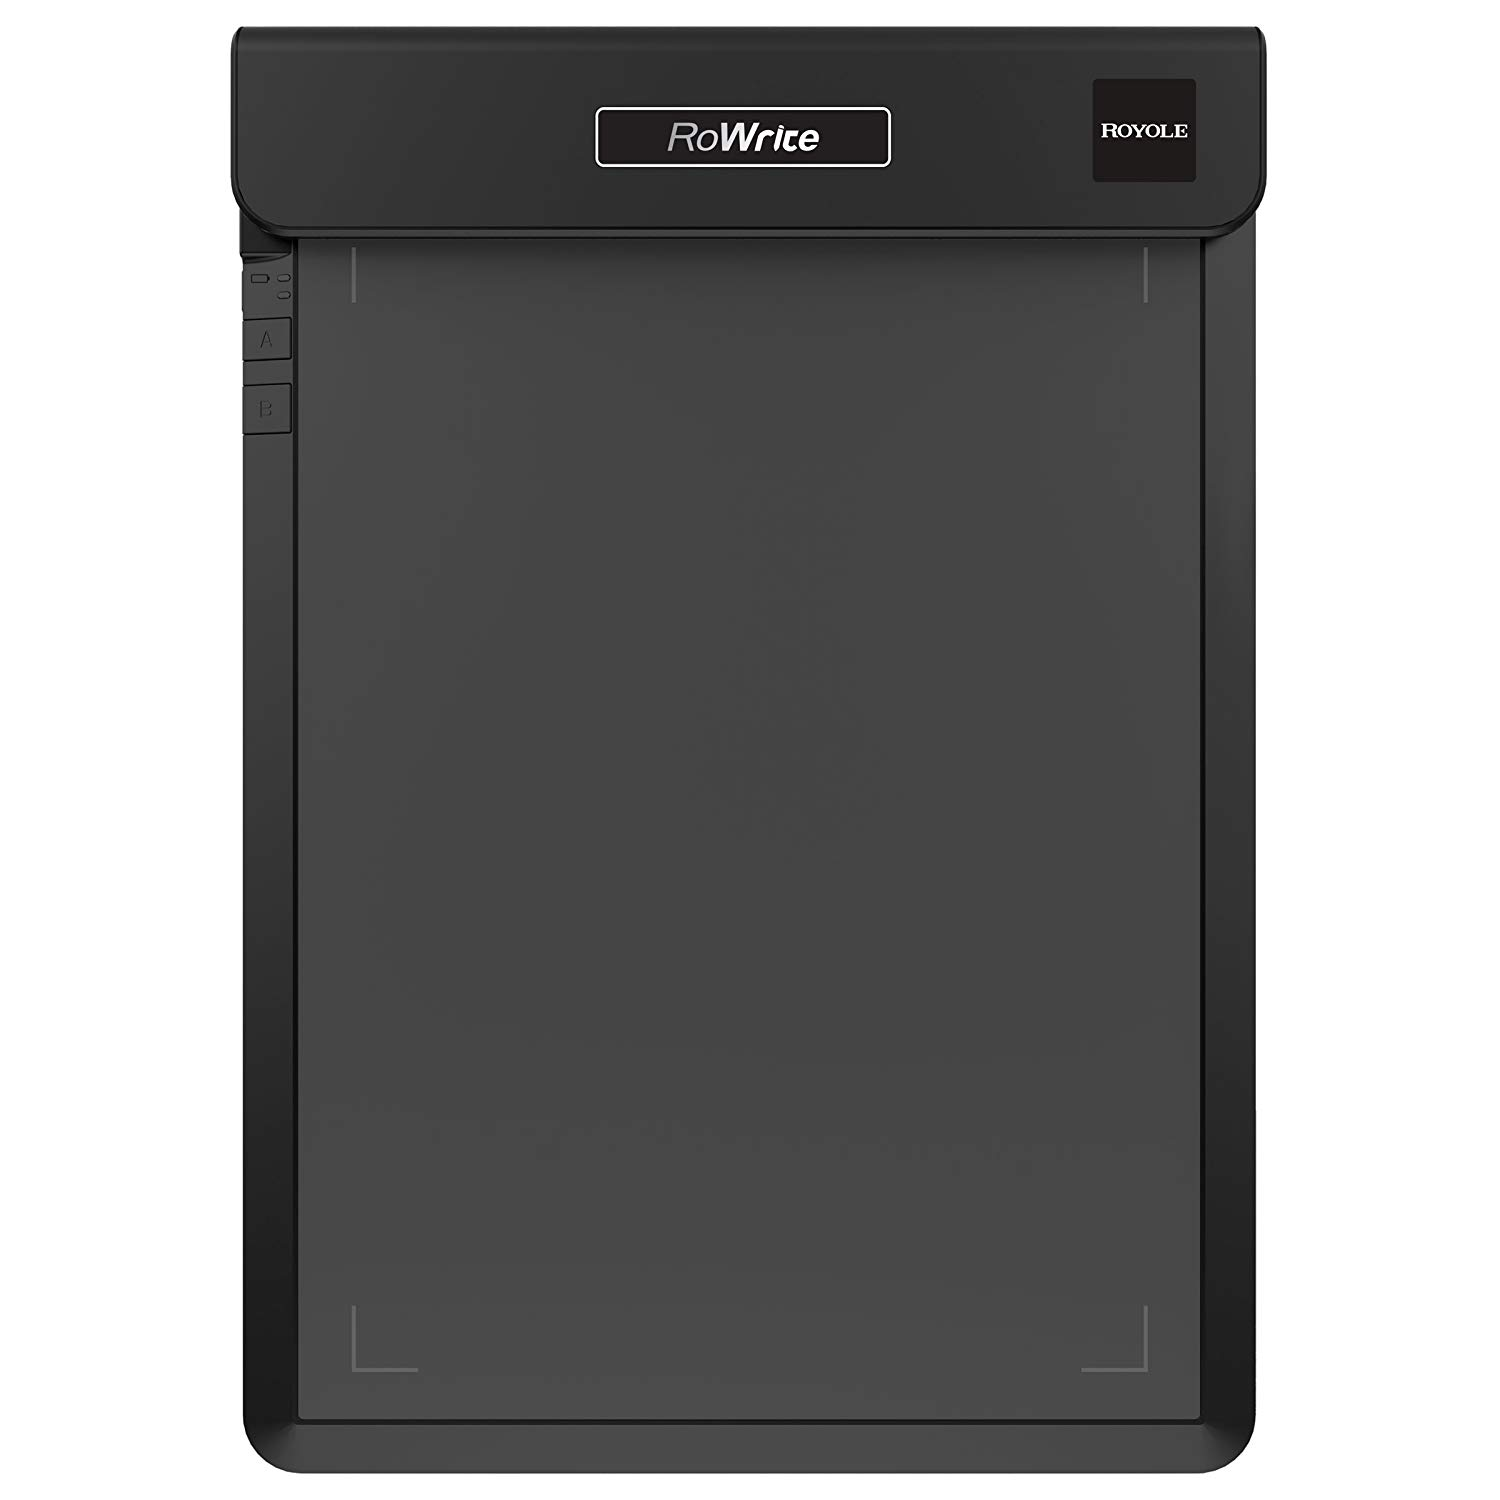
\includegraphics[width=\linewidth]{rowrite.jpg}
  \label{fig:awesome_image1}
  \caption{柔宇RoWrite笔记本,这里只显示了底板}
\endminipage
\minipage{0.50\textwidth}%
  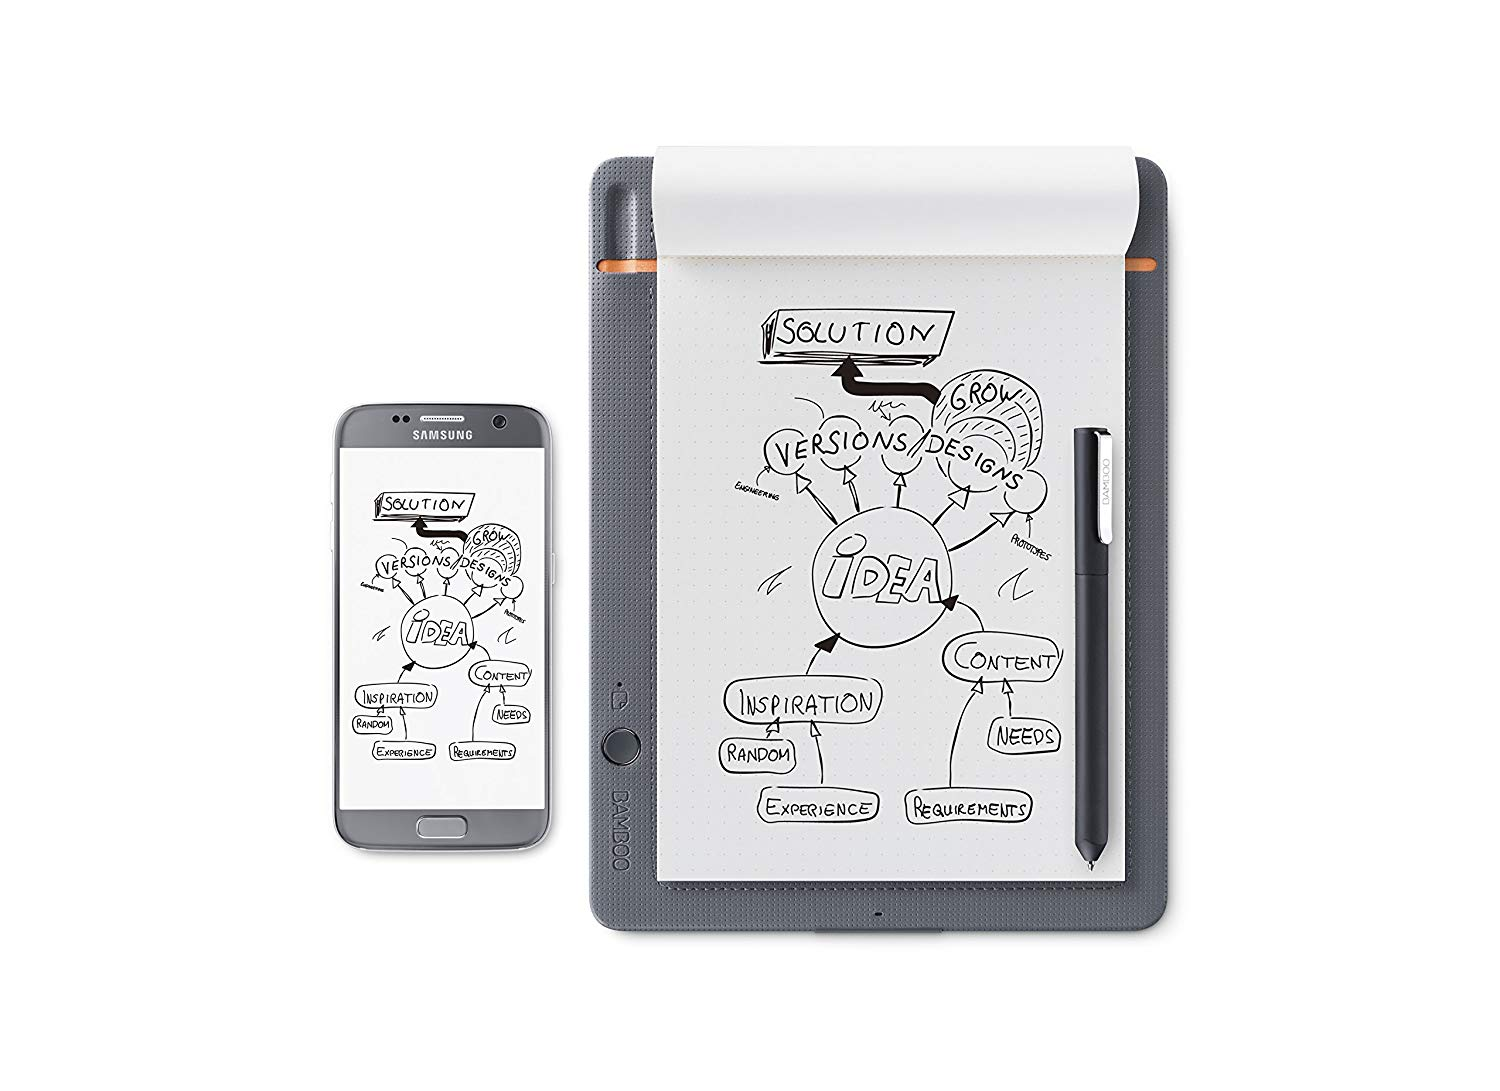
\includegraphics[width=\linewidth]{bamboo.jpg}
  \label{fig:awesome_image3}
  \caption{Wacom bamboo slate}
\endminipage
\end{figure}

\section{设想的具体实现}

图三是我的设想的原型草图。

\begin{figure}[!htb]
\minipage{1.00\textwidth}
\centering
  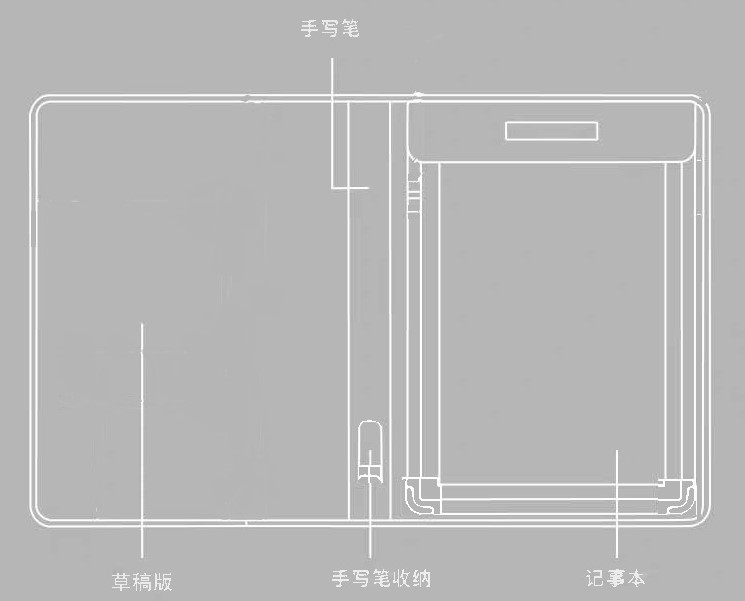
\includegraphics[width=0.8\linewidth]{prototype_fine.jpg}
  \label{fig:awesome_image1}
  \caption{设想草图}
\endminipage
\end{figure}

在左侧是一个平板,它通过内置的应用和触摸屏支持类似纸笔的记事本功能,方便在打草稿或是列算式的时候使用它。类似的功能在许多平板中都有简单的实现,或许可以直接照搬类似的应用,根据用户的使用反馈再迭代更新它。此外左侧的平板中也内置应用支持

\begin{itemize}
    \item 存储、管理、备份自己的资料
    \item 在小组(e.g. 班级、年级)中分享、获取资料
    \item 为学校管理员提供权限来增删改查资料。
\end{itemize}

这部分的实现可以参考数据中心文件系统的一种实现方式,采用master-slave架构,学校维护一个中心的服务器,每一个学生对应一个容器(container)。学生的客户端保存一个容器的镜像,在修改时和服务器同步。这样实现的一个优势是将所有学生的文件统一在一台机器之后可以 a) 便于校方的管理 b) 技术上可以利用现有的文件系统压缩重复出现的文件(e.g. 课件、作业题目)。后者的一种可行方案是利用GlusterFS和AUFS,一个简单的例子请参考脚注链接\footnote{https://github.com/DanDoge/Lab-on-Operating-Systems/tree/master/第五次作业}的后半部分。通过给每一个客户端分配ip地址,这样的设计自然的支持了各个客户端之间通过网络的资料互传,通过将每一个小组划分在一个子网内,资料的共享也可以自然的完成。

右侧的底板会使用类似bamboo slate或者柔记的技术配合特定的手写笔支持压感扫描笔记本上的内容。笔记本的部分,为了压低耗材的价格也方便使用,我们最好不要采用专用的笔记本,而最好适配所有普通的纸张。为固定笔记本以使得扫描结果的每一页绝对位置都相同,可以在上面用夹子类似的结构固定住本子。对于扫描文本的方式,除了我设想的实时扫描之外,还可以在写完一页之后整体扫描一次,替换成这样的扫描方式既能够增加扫描的精度,也或许能够降低整体成本。但这样需要在写完每一页/写完几页之后进行额外的操作,或许会使用户使用的时候意识到这是一个电子产品,而打破了传统纸笔上书写-翻页-书写-翻页的循环。另一方面,bamboo slate有类似的机制要求用户在翻页时按键开启新的一页,用户的评论\footnote{https://www.amazon.com/Wacom-Smartpad-Digital-Notebook-CDS610S/dp/B01KKPC0WA?th=1}有反应在真实书写的时候会忘记按键而需要后期再处理。

余下的部分包括
\begin{itemize}
    \item 封皮:不同于普通的笔记本封皮,在这里它需要保护里面的电子产品。它可以是牛皮纸板,或是真皮的书衣,只要耐用结实的材料都可以胜任,防水的材料更好。封皮中间的部分可以放置连接左右两部分的接线。
    \item 手写笔:现有的技术已经支持在专用的手写笔上更换笔芯,笔芯的价格也在可以承担的范围中。在中间的位置我设计了一个放笔的位置,这样不会容易丢掉手写笔。
\end{itemize}

\section{困难与解决方案}

推行上的困难我想大致包含两个方面,价格和扫描结果的准确性。前文中提到的竞品价格大多在一千元以上,因为这些产品都没有大规模推开,没有平摊研发成本,我推测成本价格大致在一千元左右,但即便是这样的价格也只意味着能在重点中学铺开,不会面向一个很大的群体。可行的压缩成本的方案包括将降低左侧平板的配置(e.g. CPU,RAM),这是考虑到它的主要操作并不会很消耗计算资源。

另一个可能的困难来自扫描结果的准确性。作为主打扫描纸质资料的产品,欠佳的扫描效果会很大降低使用满意度。一种可行的方案是利用现有的人工智能技术智能补全缺失的内容。这方面的训练数据可以通过擦除一些完整的笔记的一些部分来得到,训练简单的神经网络补全缺失的部分。

此外还需要考虑非技术性的问题,包括如何组织一个团队推行这个项目,还包括如何打入教育市场和说服教育局或是家长使用它的优越性,这方面可能需要政府方面的人脉或是特定项目的支持。

\section{总结}

在上文中,我设想了一种致力于改善学生学习体验的智能笔记本,它针对可能使用的场景和需求进行了独特的设计和优化。此外,我也探讨了它可能遇到的困难和可行的解决方案。这一个学期以来的对设计产品方面的观摩和动手实践无疑为我的设想提供了充足的背景知识,老师在课堂上指出的问题也拓宽了我思考的方向。可能未来有一天我会亲身参与类似的项目,运用到课堂上学到的知识和这次朴素的设想。但无论如何,我相信这门课上感受到的东西都会在未来的生活中派上用场的。



\end{document}
